\ifx\wholebook\relax \else

\documentclass[UTF8]{article}

\usepackage[nomarginpar
  %, margin=.5in
]{geometry}

\addtolength{\oddsidemargin}{-0.05in}
\addtolength{\evensidemargin}{-0.05in}
\addtolength{\textwidth}{0.1in}

\usepackage[cn]{../../prelude}

\setcounter{page}{1}

\begin{document}

\title{参考答案}

\author{刘新宇
\thanks{{\bfseries 刘新宇} \newline
  Email: liuxinyu95@gmail.com \newline}
  }

\maketitle
\fi

\markboth{参考答案}{编程中的数学}

\chapter*{参考答案}
\phantomsection  % so hyperref creates bookmarks
\addcontentsline{toc}{chapter}{参考答案}

\section{前言}

\begin{enumerate}
\item 编程实现一个井字棋游戏是传统人工智能中的经典问题,而计算机可以轻松算出三个数字的和并判断其是否等于15。请利用这个同构编写一个简化的井字棋程序,并做到不被人类玩家击败。

我们的思路是使用《洛书》幻方来同构井字棋游戏,我们用集合$X$, $O$来保存两个玩家所占领的格子。对于前言中的对局,开始时$X = \phi$,$O = \phi$,结束时$X = \{ 2, 5, 7, 1 \}$,$Y = \{ 4, 3, 8, 6 \}$。为此我们需要先写一个程序判断一个集合中是否有3个元素相加等于15,从而知道某个玩家获胜与否。

有两种思路解决这个问题,第一种是列举洛书幻方中的所有行、列、对角线,共8个三元组:$\{ \{4, 9, 2\}, \{3, 5, 7\}, ..., \{2, 5, 8\} \}$。然后看是否某个三元组包含在玩家占领的格子集合中。第二种比较有趣,假设玩家占领了格子$ X = \{x_1, x_2, ..., x_n\}$。这些格子按照洛书幻方中的元素升序排列。我们可以先选出$x_1$,然后用左右两个指针$l, r$分别指向下一个元素和最后一个元素,然后把这3个数加起来$s = x_1 + x_l + x_r$,如果等于15,说明玩家连成一条直线已经获胜了。如果小于15,由于元素是升序排列的,我们可以把左侧指针$l$加一,然后再次尝试;如果大于15,我们把右侧指针$r$减一,然后再次尝试。如果左右指针相遇,说明固定$x_1$没有找到相加等于15的三元组,我们选出$x_2$再次进行这样的检查。这样最差情况总共进行$(n - 2)+ (n - 3) + ... + 1$次检查就得知玩家是否获胜了。

\lstset{language=Python
    , frame=single
}
\begin{lstlisting}
def win(s):
    n = len(s)
    if n < 3:
        return False
    s = sorted(s)
    for i in range(n - 2):
        l = i + 1
        r = n - 1
        while l < r:
            total = s[i] + s[l] + s[r]
            if total == 15:
                return True
            elif total < 15:
                l = l + 1
            else:
                r = r - 1
    return False
\end{lstlisting}

这样给定$X$和$O$,就能判断局面。如果$X$和$O$占满全部9个格子,还未分出胜负,则表示平局。接下来我们用传统人工智能中的$min-max$方法来实现井字棋,我们给每个局面一个评分,一方试图让评分最大化,称为正方;另一方试图让评分最小化,称为反方,从而实现对抗。平局的话评分为0,如果某个局面让正方获胜,我们设置评分为10,反方获胜评分为-10。这个分数值完全是随意设置的,不影响结果。

\begin{lstlisting}
WIN = 10
INF = 1000

# Luo Shu magic square
MAGIC_SQUARE = [4, 9, 2,
                3, 5, 7,
                8, 1, 6]

def eval(x, o):
    if win(x):
        return WIN
    if win(o):
        return -WIN
    return 0

def finished(x, o):
    return len(x) + len(o) == 9
\end{lstlisting}

对于任何一个对局,我们都让计算机不断向前探索,直到找到输赢或者平局的确定局面才停下来。探索的方法是穷尽当前所有能占领的格子,然后转换身份,考虑自己是对方时怎样对抗。对于所有候选方案,如果是正方,就选择评分高的方案,如果是反方,就选择评分低的方案。

\begin{lstlisting}
def findbest(x, o, maximize):
    best = -INF if maximize else INF
    move = 0
    for i in MAGIC_SQUARE:
        if (i not in x) and (i not in o):
            if maximize:
                val = minmax([i] + x, o, 0, not maximize)
                if val > best:
                    best = val
                    move = i
            else:
                val = minmax(x, [i] + o, 0, not maximize)
                if val < best:
                    best = val
                    move = i
    return move
\end{lstlisting}

$min-max$是一个递归搜索的过程,为了尽快获胜,我们在评分上加上对向前探索步数的考虑。如果是正方,就从评分中减去递归深度,而对于反方,则加上递归深度。

\begin{lstlisting}
def minmax(x, o, depth, maximize):
    score = eval(x, o)
    if score == WIN:
        return score - depth
    if score == -WIN:
        return score + depth
    if finished(x, o):
        return 0  # draw
    best = -INF if maximize else INF
    for i in MAGIC_SQUARE:
        if (i not in x) and (i not in o):
            if maximize:
                best = max(best, minmax([i] + x, o, depth + 1, not maximize))
            else:
                best = min(best, minmax(x, [i] + o, depth + 1, not maximize))
    return best
\end{lstlisting}

现在我们就做出一个无法被人类击败的程序了,我们的程序在背后用洛书幻方对抗人类玩家:

\begin{lstlisting}
def board(x, o):
    for r in range(3):
        print "-----------"
        for c in range(3):
            p = MAGIC_SQUARE[r*3 + c]
            if p in x:
                print "|X",
            elif p in o:
                print "|O",
            else:
                print "| ",
        print "|"
    print "-----------"

def play():
    x = []
    o = []
    while not (win(x) or win(o) or finished(x, o)):
        board(x, o)
        while True:
            i = int(input("[1..9]==>"))
            if i not in MAGIC_SQUARE or MAGIC_SQUARE[i-1] in x or
               MAGIC_SQUARE[i-1] in o:
                print "invalid move"
            else:
                x = [MAGIC_SQUARE[i-1]] + x
                break
        o = [findbest(x, o, False)] + o
    board(x, o)
\end{lstlisting}

\end{enumerate}

\section{自然数}

\begin{enumerate}
\item 定义0的后继为1,证明对于任何自然数都有$a \cdot 1 = a$

首先用数学归纳法证明$0 + a = a$这个结论,见附录I。然后:
\[
\begin{array}{rlr}
a' \cdot 1 & = a' \cdot 0' & \text{定义0的后继为1} \\
           & = a' \cdot 0 + a' & \text{乘法定义规则二} \\
           & = 0 + a' & \text{乘法定义规则一} \\
           & = a' & \text{此前证明的结论}
\end{array}
\]

\item 证明乘法分配律

可以用数学归纳法证明左侧的分配律$c(a + b) = ca + cb$。首先是$b = 0$的情况:

\bre
c(a + 0) & = & ca & \text{加法规则一} \\
         & = & ca + 0 & \text{反向用加法规则一} \\
         & = & ca + c0 & \text{反向用乘法规则一} \\
\ere

递推假设$c(a + b) = ca + cb$,接下来证明$c(a + b') = ca + cb'$

\bre
c(a + b') & = & c(a + b)' & \text{加法规则二} \\
          & = & c(a + b) + c & \text{乘法规则二} \\
          & = & ca + cb + c & \text{递推假设} \\
          & = & ca + (cb + c) & \text{加法结合律} \\
          & = & ca + cb' & \text{反向用乘法规则二} \\
\ere

\item 证明乘法结合律和交换律

我们只证明乘法结合律$(ab)c = a(bc)$,乘法交换律的证明则给出一个提纲。利用数学归纳法,首先是$c = 0$的情况:

\bre
(ab)0 & = & 0 & \text{乘法规则一} \\
      & = & a0 & \text{反向用乘法规则一} \\
      & = & a(b0) & \text{反向用乘法规则一} \\
\ere

递推假设$(ab)c = a(bc)$,接下来要证明$(ab)c' = a(bc')$

\bre
(ab)c' & = & (ab)c + ab & \text{乘法规则二} \\
       & = & a(bc) + ab & \text{递推假设} \\
       & = & a(bc + b) & \text{上题证明的分配律} \\
       & = & a(bc') & \text{反向用乘法规则二} \\
\ere

证明乘法交换律可以分为三步,都使用数学归纳法。首先证明$1a = a$,然后再证明右侧的分配律$(a + b)c = ac + bc$,最后再证明交换律。

\item 如何利用皮亚诺公里验证3 + 147 = 150

我们先看看经典的2 + 2 = 4是怎么证明的:

\bre
2 + 2 & = & 0'' + 0'' & \text{2是0的两次后继} \\
      & = & (0'' + 0')' & \text{加法定义规则二} \\
      & = & ((0'' + 0)')' & \text{加法定义规则二} \\
      & = & ((0'')')' & \text{加法定义规则一} \\
      & = & 0'''' = 4 & \text{0的4次后继} \\
\ere

显然用这个方法证明3 + 147 = 150的话太冗长了,我们可以用先前证明的加法交换律证明147 + 3 = 150会容易一些。另一个方法是通过数学归纳法证明$3 + a = a'''$。

\item 试给出乘法分配律,乘法结合律,和乘法交换律的几何解释。

\begin{figure}[htbp]
 \centering
 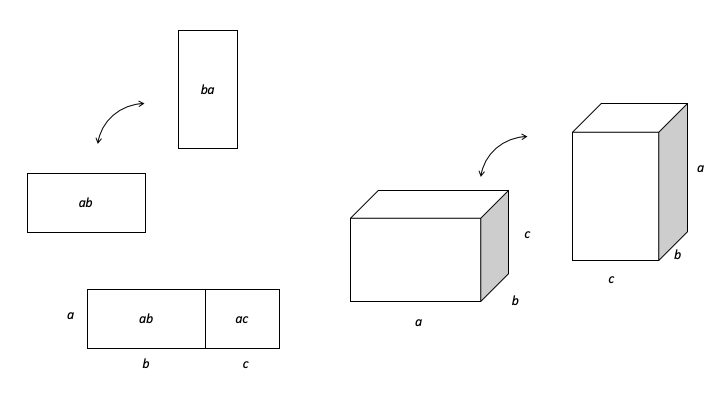
\includegraphics[scale=0.4]{img/geometric-arithmetic.png}
 \captionsetup{labelformat=empty}
 \caption{乘法交换律、结合律、分配律的几何解释}
 \label{fig:geometric-arithmetic}
\end{figure}


\item 使用$foldn$定义平方$()^2$。

可以利用递推关系$(n+1)^2 = n^2 + 2n + 1$来定义平方:

\[
()^2 = 2nd \cdot foldn\ (0, 0)\ h
\]

其中$h$接受一对值$(i, s)$,分别代表自然数$i$和它的平方$s$。它将第一个值递增1,然后利用平方展开式求出下一个平方数。

\[
h\ (i, s) = (i + 1, s + 2i + 1)
\]

\item 使用$foldn$定义$()^m$,计算给定自然数的$m$次幂。

一种简单的方法是借助第一章中定义的$m^{()} = foldn(1, (\cdot m))$来定义$()^m$:

\[
()^m = 2nd \cdot foldn\ (0, 0)\ h
\]

其中

\[
h\ (i, b) = (i + 1, (i + 1)^m)
\]

这看起来有些奇怪,所有中间计算都被直接丢掉了。另一种方法是利用牛顿二项式定理:

\[
(n + 1)^m = n^m + \binom{m}{1} n^{m-1} + ... + \binom{m}{m-1} n + 1
\]

这样就建立了递推关系:

\[
(n)^m = 2nd(foldn\ (1, 1)\ h\ (n - 1))
\]

其中

\[
h (i, x) = (i + 1, C \cdot X)
\]

这里$C \cdot X$是二项式系数和各次幂的点积$C \cdot X = \sum c_j x_j$。各次幂可以通过对$x$不断除以$i$求出,二项式定理的系数可以由帕斯卡三角形逐行递推得到。下面是综合在一起的例子程序:

\lstset{language=Haskell
    , frame=single
}
\begin{lstlisting}
exp m n = snd $ foldn (1, 1) h (n - 1) where
  cs = foldn [1] pascal m
  h (i, x) = (i + 1, sum $ zipWith (*) cs xs) where
    xs = take (m + 1) $ iterate (`div` i) x

pascal = gen [1] where
  gen cs (x:y:xs) = gen ((x + y) : cs) (y:xs)
  gen cs _ = 1 : cs
\end{lstlisting}

\item 使用$foldn$定义奇数的和。它会产生怎样的序列?

用$foldn$定义1 + 3 + 5 + ...为$2nd \cdot foldn\ (1, 0)\ h$,其中:

\[
h\ (i, s) = (i + 2, s + i)
\]

如第一章中的插图所示,奇数和总是平方数。

\item 地面上有一排洞,一只狐狸藏在某个洞中。每天狐狸会移动到相邻的下一个洞里。如果每天只能检查一个洞,请给出一个捉到狐狸的策略,并证明这个策略有效。如果狐狸每天移动的不止一个洞呢?

\end{enumerate}

\section{递归}

\section{无穷}

\begin{enumerate}
\item 数论中的算术基本定理说:任何一个大于1的整数都可以唯一地表示成若干素数的乘积。有一道编程趣题,要求判断一段文字$T$中,是否包含一个字符串$W$的某种排列。试利用算术基本定理,和素数流解决这道题目。

我们的思路是,将每一个不同字符对应到一个素数上去,a对应2,b对应3,c对应5……。这样任意给定一个字符串$W$,不管它是否包含重复的字符,我们都可以把它表示为素数的乘积:

\[
F = \prod p_c , c \in W
\]

我们称其为字符串$W$的数论指纹$F$。如果$W$是空串,我们规定它的指纹等于1。根据整数乘法的交换律,我们知道无论$W$怎样排列,其数论指纹都不变,并且根据算术基本定理,这个数论指纹是唯一的。现在我们就得到了一个特别简洁的解法:我们首先计算出$W$的数论指纹$F$,然后用一个长度为$|W|$的窗口沿着$T$从左向右滑动。一开始我们需要计算$T$在这个窗口内的数论指纹,并和$F$比较,如果相等就说明$T$包含$W$的某种排列。如果不等我们将这个窗口向右滑动一个字符。此时我们可以非常容易地计算新窗口内的数论指纹:只要把滑出的字符对应的素数除掉,再把滑入的字符对应的素数乘上就可以了。任何时候如果新窗口内的数论指纹等于$F$,就说明找到了一个排列。当然为了获得每个不同字符对应的素数,我们还要利用埃拉托斯特尼筛法产生一串素数。下面是一段示例算法:

\begin{algorithmic}
\Function{contains?}{$W, T$}
  \State $P \gets ana \ era \ [2, 3, ...]$ \Comment{素数序列}
  \If{$W = \phi$}
    \State \Return True
  \EndIf
  \If{$|T| < |W|$}
    \State \Return False
  \EndIf
  \State $\displaystyle m \gets \prod P_c, c \in W$
  \State $\displaystyle m' \gets \prod P_c, c \in T[1...|W|]$
  \For{$i \gets |W| + 1$ to $|T|$}
    \If{$m = m'$}
      \State \Return True
    \EndIf
    \State $m' \gets m' \times P_{T_i} / P_{T_{i - |W|}} $
  \EndFor
  \State \Return $m = m'$
\EndFunction
\end{algorithmic}

\end{enumerate}

\ifx\wholebook\relax \else

\expandafter\enddocument
%\end{document}

\fi
